\chapter{Quantum Internet}

In this chapter, we conclude the book with a discussion of extending from the technologies we have developed throughout the book to a full \emph{Quantum Internet}, a global network of quantum networks. We also give some thoughts about developing \emph{standards} for quantum communications, and how understanding quantum communication can lead to a variety of careers in quantum. This chapter is presented as a dialog between the two main authors, edited for clarity.

\section{Networks of networks}

\rrr (laughing) Michal, you look so serious!

So, welcome to chapter fifteen: Quantum Internet.

Up until this point, I've been behind the camera instead of in front of it, but we thought we'd do this last chapter together.

\mmm So, what is the Quantum Internet?

\rrr I don't know, let's find out. 

\mmm Let's find out!

Let's begin with Step One: Network of Networks.

This is a combination of words that you've been hearing quite a lot throughout this module, and here we will give you a slightly more concrete idea of what it really means.

\rrr So first off, the Internet is this really complicated thing. There are a whole bunch of individual networks, and a whole bunch of individual nodes that make up each network. So the global Internet is a "network of networks". Let's see a little bit about how that works.

\begin{figure}[t]
    \centering
    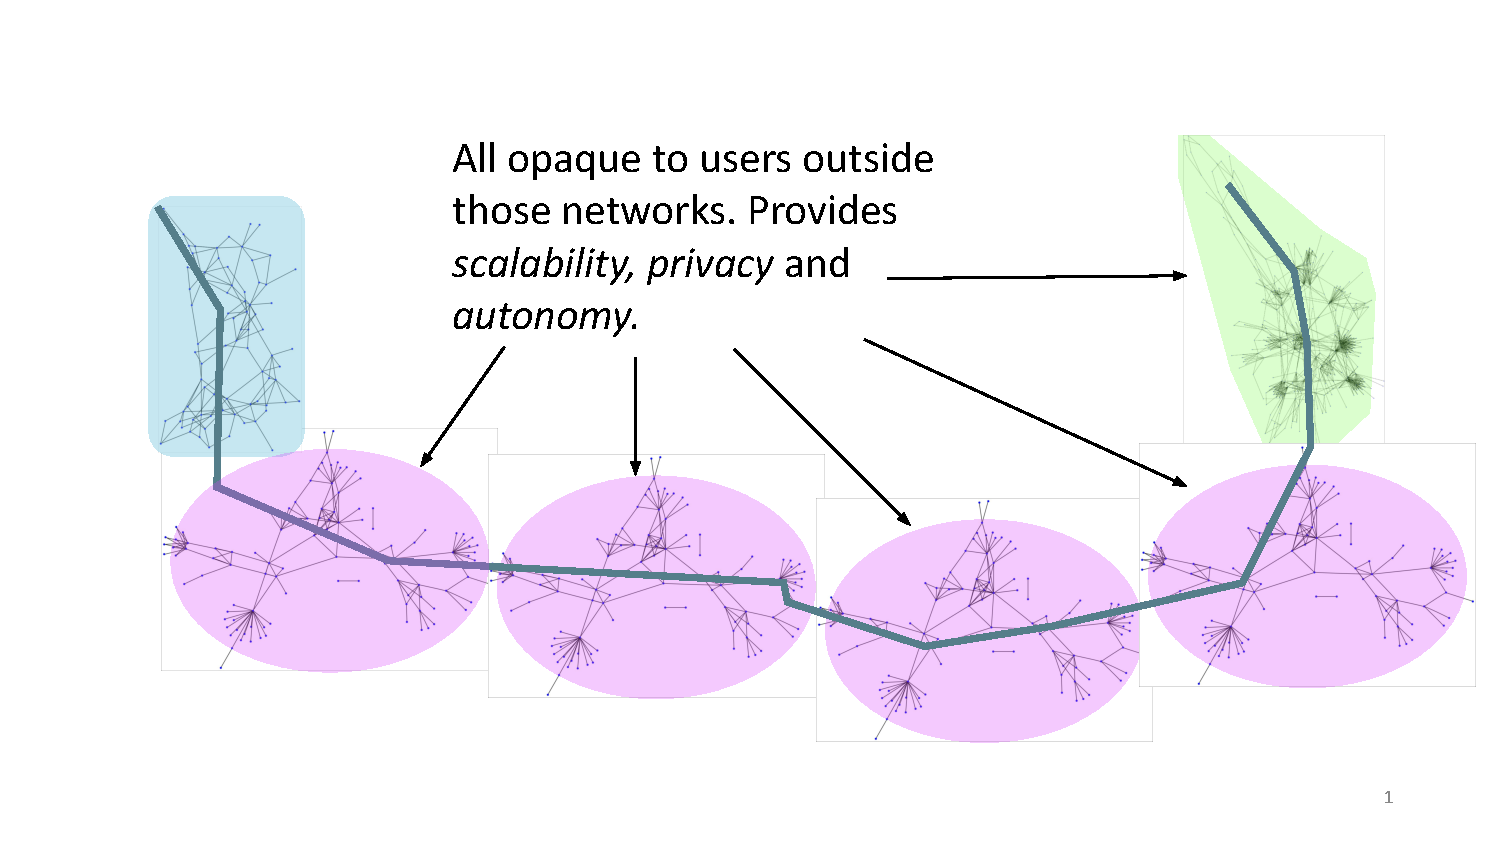
\includegraphics[width=1\textwidth]{lesson15/R2L15fig1.pdf}
    \caption[Network of Networks]{Across an internetwork, a connection passes through many separate, independently managed networks that cooperate with each other for communication purposes.  The internal structure of each network is opaque to any node that is not a member of that network; outsiders know only that the network agrees to facilitate communication between neighboring networks.}
    \label{fig:15-1-NofN}
\end{figure}


Let's see, assume you want to start in the upper left-hand corner of Fig.~\ref{fig:15-1-NofN}. Your home network is the blue network, and you want to connect to some service that's out on the green network, and you have to get there through the series of pink networks. Michal, how are we going to get there?

\mmm Well, we don't actually know, because we are on the blue network, we just tell the Internet, "get us there" and magically it happens!

\rrr Okay, so let's see. So what happens next? We have this path that we've sketched out here on this arbitrary sort of network here, but the reality is that you're connected to one network and your traffic is going to go from your current location to what's called a \emph{gateway}\index{gateway} to the outside world, also called a \emph{border router}\index{border router}, and then from there it's going to hop across some other networks to get to where it wants to be, right? But, in order to make the whole system work, you don't know anything about the inside of those other networks. You only know about the blue network.

The other networks are all opaque to the users that are outside. If you are the operator of one of these networks, this opacity provides you with \emph{scalability}, \emph{privacy}, and \emph{autonomy}. Scalability is crucial, of course --- otherwise, how are we going to get to billions and billions of nodes on the internetwork?

\mmm (True!)

\rrr You can't- you can't have every single node on the network know everything about every other node on the entire network, it can't scale it that way. But it's also true that the people who own networks want to be able to evolve what's inside the network at their own rate, using potentially their own choices of technology and changing what's going on on the inside, and they don't want to share that information outside for business reasons, or for privacy reasons, you know for competitive advantage reasons or whatever, and this gives us a certain amount of autonomy, right? So in this network, you'll see there are, you know, your network, the blue one, and you have to know how to get across your network to that gateway, and then the gateway has to know which network to send things to next. But it doesn't have to know anything about the inside of those. All right, so let's see what's next.

\mmm Let's have a look where the classical Internet is right now. As of March of 2021, where this was recorded, there are around seventy one thousand autonomous systems.

\rrr So what's an autonomous system?

\mmm I was going to ask the same question!

\rrr An autonomous system is one of those networks that was one of the pink ones, or one of the blue ones, or one of the green ones in the figure. Roughly, you can think of an autonomous system as corresponding to an organization, so Keio University would have one network, it's one autonomous system, the WIDE Project would have one network that's one autonomous system, and the routing protocol then knows which network to go to next, which one of these autonomous systems to go to next.

\mmm So, there's around 870,000 IPv4 routing table entries. What does that actually mean? Can you put that into perspective? It sounds like a large number but what really does it mean?

\rrr It does! So what it means is there are 870,000 relationships between pairs of networks out of those 71,000 networks above there, so roughly so you know twelve or fourteen connections per network. On average, this means that each one of those pink or blue or green networks on average is going to be connected to about a dozen other networks. These connections may be direct between two networks (known as \emph{private peering}), or shared with several networks at places that are called \emph{Internet exchange points}, or IXPs or sometimes just IXes\index{Internet exchange point (IXP)}.

\mmm (Right.)

\rrr So collectively, each one of those, they show up in the overall structure for routing across the entire planet, and that entire set of routes is how you figure out how to get from your own network to whatever service you're trying to connect to somewhere on the other side of the planet.

\mmm You know what that reminds me of? 

\rrr What?

\mmm Of the previous animations that we had of the completely connected graph, where we said it doesn't make sense to just connect all of the nodes to all of the other possible nodes in in the network. Same here, (Exactly!) you see- you said there's exactly around 12 to 14 connections between the autonomous systems, it's the same logic, right?

\rrr Yeah! So actually, if you took that whole 71,000 networks and connected every network to every in a \emph{complete graph}...how many connections would that be?  What's 71,000 squared divided by two? That would be... 5 billion divided by 2, so two and a half billion entries instead of about a million. If every network directly was capable of exchanging traffic with it with every other network, but the reality is that they don't, right? Now the whole evolution of how the Internet got this way and how many of these networks there are, and the organization of them- which ones connect to each other's- a lot of that comes from historical business relationships and the like, and the quantum internet will probably evolve in a very different fashion, but this same general idea of having networks that are owned and operated by an organization and they connect to other networks, that same idea is going to stay.

\mmm I can imagine that, I mean developing quantum technology is a very expensive business, so you don't just give access to anybody to everything that you have spent so much money in developing and researching.

\rrr Yeah! Well, and so, and the next point right here, so there are already billions of nodes connected to the network- we talked about that in one of the earlier steps- computers and mobile phones and IoT devices, and there is no central node registry, so the true number of these things isn't known. So if you run a network, you can put more devices on the network subject to you know certain constraints- do you have the ability to give them addresses and send their traffic out to places and things like that, but this general idea really holds for that, as opposed to the phone system where there is a central authority that gives out phone numbers, and so there's somebody who could actually count all of the phone numbers and tell you where they are and you can figure out how many phones there are, but with the Internet, who knows how many devices are actually connected to it? And it's because of the autonomy provided by that system where each of the individual networks is allowed to control what goes on inside of its own network.

\mmm That sounds like a very clever system, it must have taken quite some time to develop this system, no?

\rrr Well, you know, half a century or so since the earliest ARPANET experiments, but let's see, so when did this real sort of system of autonomous networks and other protocols, including, so one of the things that's mentioned here on the slide that we haven't mentioned yet is BGP, that's the border gateway protocol and that is the protocol that exchanges this information about the relationships between those networks. When did all of that develop? Well, you know, I'd have to go back and look to be sure, but the late 80s and early 90s is pretty much when this structure was laid out.

\mmm So where do you think the quantum Internet is in relation to the classical Internet?

\rrr We're still decades and decades away.

\mmm (Right.) 

\rrr from reaching this kind of scale, but we want to apply what we have learned over the last half century in the process of developing the classical internet, and use that knowledge to actually design and develop the quantum internet as we go.

\mmm Interesting...

\rrr All right, so one of the other topics that we haven't talked about yet, that's a big trend in classical information system structures, and or systems in general, including both the internet and how computing systems work and and whatnot, is virtualization. In the process of virtualization, a computer or even a network might not correspond exactly to a single physical system. So you might have a virtual server, that's really a collection of software and data, that you think is running on a particular piece of hardware but it might not actually be running here, it might be running over there instead, somewhere else. So it might pretend to be the top part of that network but it might really be somewhere down lower, and there are a lot of mechanisms built into the classical internet to make that virtualization possible, so that services can appear in multiple places and the copies of them can be in different places, and that allows the services to kind of migrate around. (Right.) And this virtualization brings a lot of benefits. We're still a long ways away from wanting something like that virtualization for the quantum internet, but maybe, eventually we'll get there. But a related concept is recursion!


\begin{figure}[t]
    \centering
    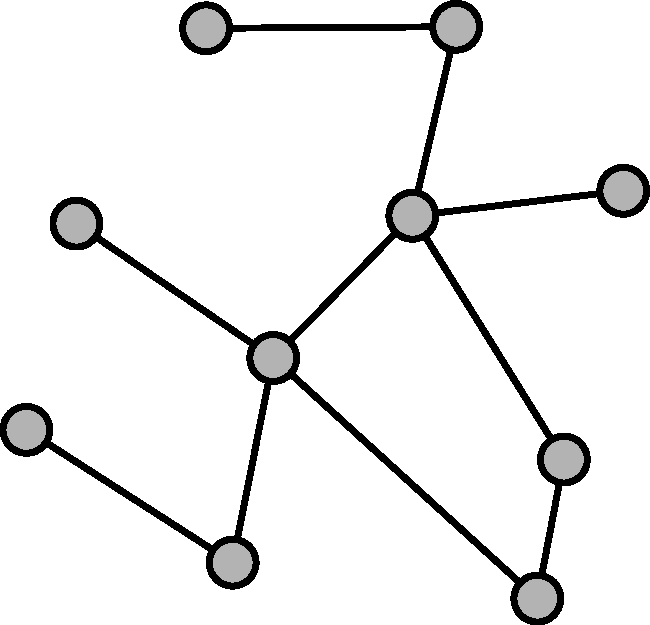
\includegraphics[width=0.5\textwidth]{lesson15/R2L15fig2.pdf}
    \caption[A simple network]{A simple network.}
    \label{fig:15-2-simple}
\end{figure}

\begin{figure}[t]
    \centering
    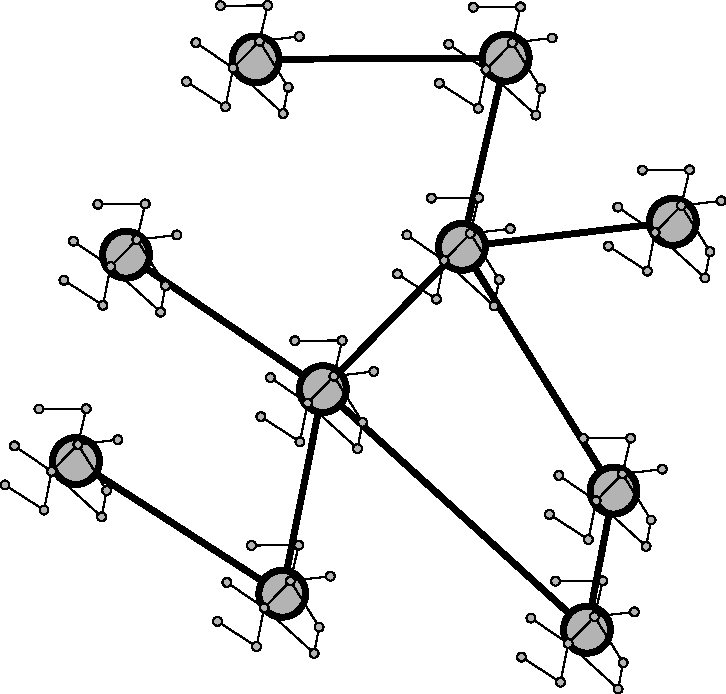
\includegraphics[width=.5\textwidth]{lesson15/R2L15fig3.pdf}
    \caption[A recursive network]{A recursive network. In this representation, each "node" in the graph is actually an abstraction of an underlying physical network, represented by the smaller nodes and links. In classical Internet terms, the larger nodes and graph could be the graph of autonomous systems.  In a  recursive network, two layers are shown here but the recursion could go deeper.}
    \label{fig:15-3-recursive}
\end{figure}

\mmm Oh recursion, I know, I remember from my computing classes.

So we said that the Internet is a network of things, where every network can be thought of as a single node of some other different layer of a network. Is that what recursion is in the context of networks? (Yeah!)

\rrr So in that earlier figure that we had with the blue network, and four or five pink networks, and the green network, each one of those inside has a structure but we can also talk about the graph that connects each of those, and so you can think about that as the recursion in the system, so the BGP system that was talking about a minute ago is essentially two layers or two tiers: there's the internal and the external protocol for connecting it, and so the internal is for how do you get around inside of your own network, and you actually have the choice to use a different protocol or a different algorithm for routing inside your network, as long as you can meet your contractual obligations with others to exchange information with them and to carry traffic back and forth across your network in some reasonable way. But then, there's the external BGP, and that's the graph of the relationship between those autonomous systems, the internet-level total architecture between the whole thing. So that's two levels, but the reality is that in most modern local area networks, there's actually another sort of routing system that's built into local area networks as well, so we've already got three layers. Conceptually, this process could actually be repeated indefinitely and we can build, what's called a recursive network.

\mmm Kind of like this right? 

\rrr (Yeah!) 

\mmm Where each node is really a different network.

\rrr Yeah, so each one of these individual nodes might be a network inside of it and then inside of that, each one of those nodes might, in turn be a network inside of that, and so conceptually at least, it could go to sort of arbitrary depth in this, and again that gets a scalability in what we're actually building, and it allows us to reuse a lot of the mechanisms that we're designing and building at the level of, you know, the global internet and then some wide area network, and then some organizational network, and then some local area network, and then possibly, even inside the individual machines you can actually use similar techniques, and sometimes, not often, but sometimes, you'll actually have a virtual network inside of your actual own machine that actually reuses some of those concepts inside, and there's no reason why that process can't just continue.

\mmm Very cool!

All right, that concludes the first step. Let's see what awaits us in the next step.

\section{Integration with classical systems}
\label{sec:classical-integration}


\mmm Rod, the title of this step is "integration with classical systems". Does that mean that the quantum internet is not going to replace the classical internet?

\rrr That's a good question, but yes, the quantum internet will not replace the classical internet! There will be two networks.

\mmm Right, so how are they going to talk to each other? How are they going to integrate together?

\rrr Let's see, so on this diagram here, we have what says quantum network, and an IP network. What's the quantum network do?

\mmm Well, we've seen that in a number of chapters here, the main purpose is to distribute entanglement between parties, whether it be bipartite entanglement, multipartite entanglement, so that it can be used as a resource for communication tasks such as teleportation and QKD, whether it's entanglement-based or single photon-based.

\rrr And QKD is, in fact, the example that's written here on the diagram, so the QKD devices, what are they doing across across the quantum network? Remind us, what's the service they provide?

\mmm Well, the thing that they're trying to do is they're trying to establish a secret correlated key between one communicating party and the other one without any eavesdropper knowing what the key is.

\rrr Right, so what's a key in this context? The key is-

\mmm The key is a secret a bit of strings, classical bit of strings, that we can use to hide our message.

\rrr All right, so it's a string of random bits that are guaranteed to be secret based on what we've done so far. So what we want to do, once we have those is to use them-

\mmm Ah, they're classical bits!

\rrr Yes they're classical bits,

% \mmm Yes, no no no no no

% \rrr Okay good

\mmm That's why we can use them with the classical internet.

\rrr Yes! So in fact, that's what we're going to do next, is we're going to actually use them with the classical internet. So the first job that happens is the quantum network makes those keys, and it makes those classical bits out of it, and then it's going to share those bits with a couple of boxes that are connected to an IP network that are called IPsec gateways, and there will be one of those at each end. Have you heard of IPsec?

\begin{figure}[t]
    \centering
    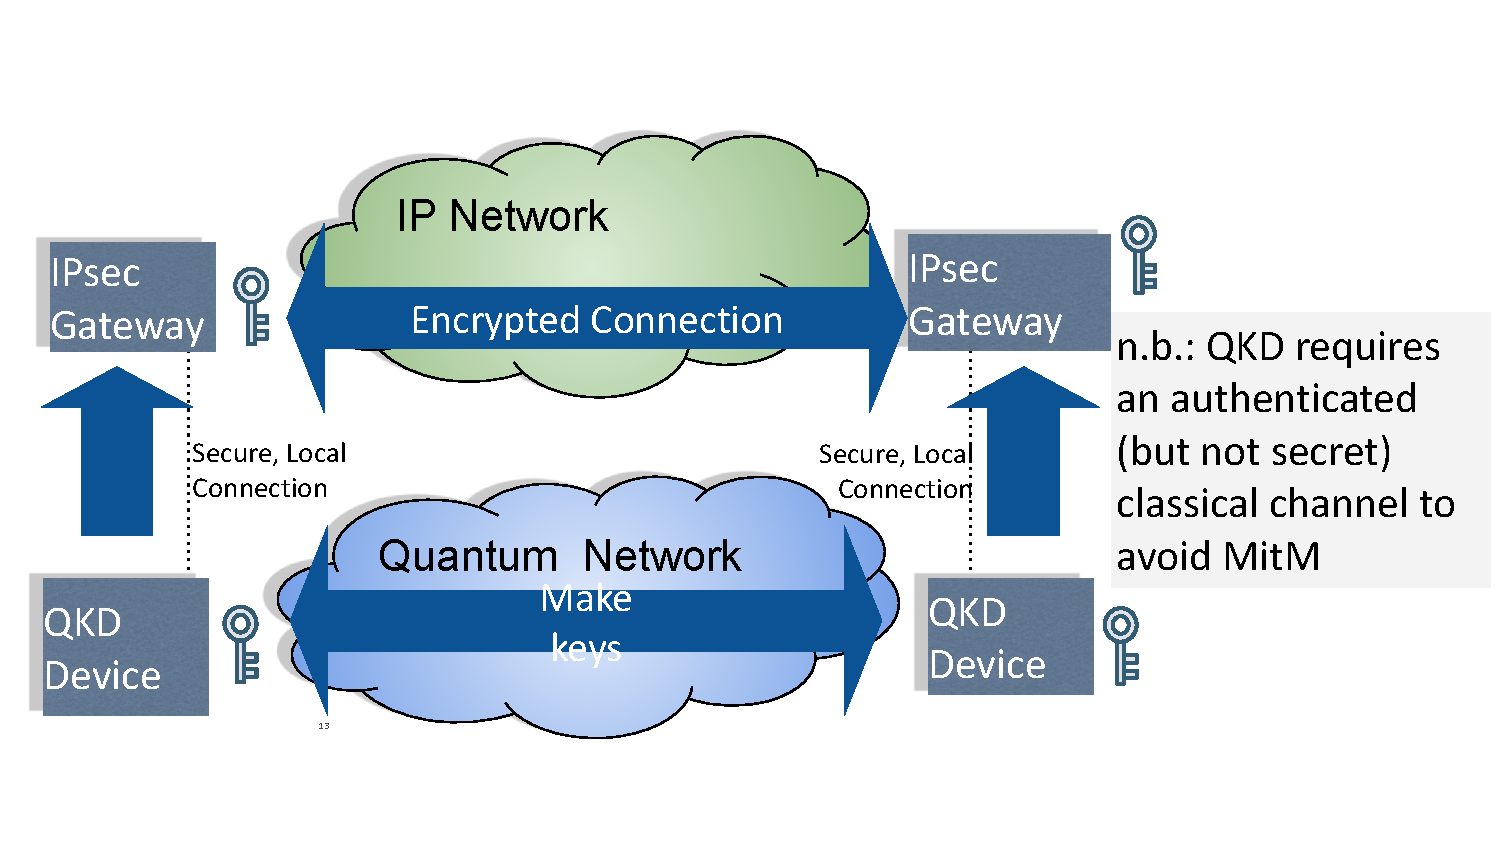
\includegraphics[width=1\textwidth]{lesson15/R2L15fig4.pdf}
    \caption[IPsec with QKD]{The Internet standard encryption protocol known as IPsec can be adapted to use keys generated via QKD rather than Diffie-Hellman key exchange.}
    \label{fig:15-4-ipsec-with-qkd}
\end{figure}

\mmm Not really, no.

\rrr IPsec is one of the standard internet protocols for how you encrypt data that you're going to share across the network. One of the other famous protocols is a protocol that's called TLS, which is used for web browsing and for a lot of other things. IPsec is actually slightly older than TLS, and its original design was to connect one network to another network securely, and so you send data to your nearby IPsec gateway and it encrypts the data and sends it to another IPsec gateway at the other end, where it gets decrypted and sent to your partner over there. So, it's a standard protocol for doing that. Now, so once we have the keys to the IPsec gateways,

before QKD, the way that these IPsec gateways work together is they have to negotiate a a key exchange of some sort, so we talked in the encryption chapter about three phases of an encrypted conversation, right? There was authentication, key generation and then the bulk data encryption.

\mmm Right.

\rrr So, the authentication is often done using public key, the key generation prior to QKD was primarily done using a mechanism called \emph{Diffie-Hellman key exchange}\index{Diffie-Hellman key exchange}, so that's what we're going to replace with the QKD, and then that data will be used to- actually that key that comes out of the QKD network or the quantum internet and the QKD devices attached to it- will be used to create the keys that are used by the IPsec gateways for encrypting large amounts of data which gets sent using an encryption mechanism, well most commonly, these days an encryption mechanism called AES, the advanced encryption standard. So, that's (see slide)- so you get this encrypted connection, and yeah, it's important to note here that the QKD connection itself actually requires that you also have an authenticated classical channel between the nodes in order to prevent someone standing in the middle of the network and pretending to be Alice in one direction and pretending to be Bob in the other direction, and that's what's called a "man in the middle attack", and we want to try to get rid of- try to avoid having that happen.

\mmm I see, so let me get this straight. The role of the quantum network really is just one step in the whole number of steps during a secret communication.

\rrr Exactly.

\mmm So we start classically, we authenticate classically, but then when we require the generation of the key, that's where the quantum part comes in, that's where the quantum magic happens, either through non-fully distinguishable states such as we saw in the BB84 protocol, or entanglement based quantum key distribution using the E91 protocol.

\rrr Right.

\mmm And whatever the result of that is, it should be a secret correlated key that's not known to any other malicious party which then gets passed back into the classical network, and we proceed classically again.

\rrr Exactly! 
% (good!)

And so all of this put together makes for an integrated quantum and classical system.

So, you're the expert on a couple of these other things that we might want to do, right?

\begin{figure}[t]
    \centering
    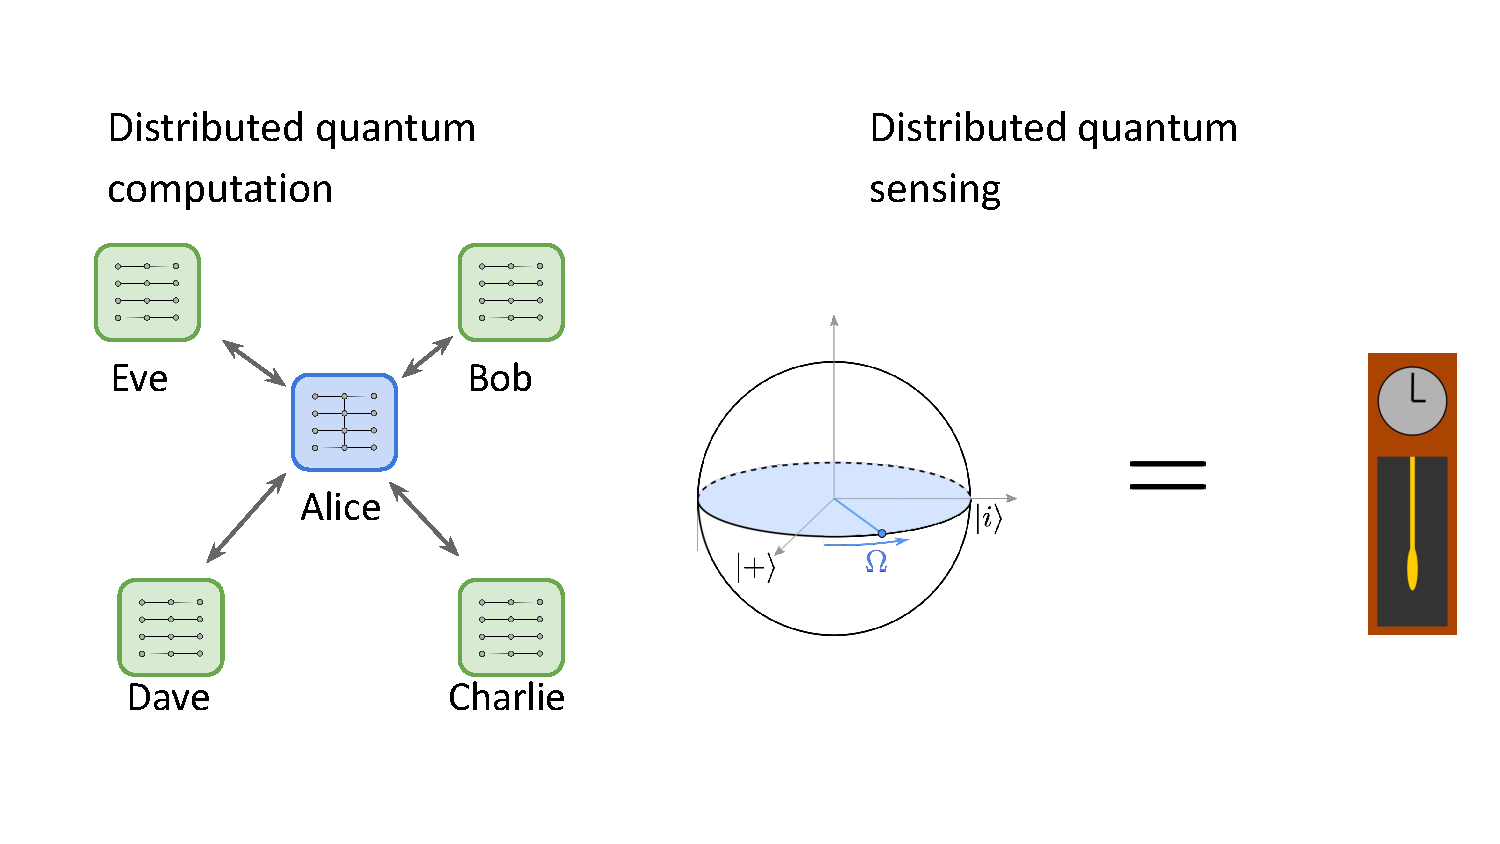
\includegraphics[width=1\textwidth]{lesson15/R2L15fig5.pdf}
    \caption[Uses of quantum networking]{Quantum networks will be used for distributed quantum computation (left) and sensing applications such as clock synchronization (right).}
    \label{fig:15-5-apps}
\end{figure}


\mmm Oh yeah, yeah, we've- we've talked about distributed quantum computation where Alice, Bob, Eve, Dave and Charlie, they share some quantum resources, but individually they cannot perform the computation that they want to, they don't have enough quantum power. So they have to figure out how to share this quantum power with each other, and to create something that allows them then, to tackle much larger quantum problems. So for that, again they have to share some quantum resources that's done by the quantum network, but then they have to coordinate with classical messages using the classical network what they need to perform, they basically use the classical control provided by the classical network to then, perform the quantum computation on the quantum part of their memories, their processors, and so on.

\rrr So in that case, this network of quantum computers that's going to do this distributed computation, is that distributed computation- is that a complete application? Is that, like, quantum photoshop or or quantum oracle database or something? Or-

\mmm Well, I would say, "never say never", but for now the problems that we envision tackling with quantum stuff are things that are genuinely quantum, where classical computers can help but are too slow, for example diagonalizing large matrices, finding new properties of new drugs, new materials, and so on. I don't think that there will be an application of a quantum Photoshop where we can- I don't even know how that would work in reality.

\rrr I don't either! So the chemistry one's a really good example, because as I understand it, there will be some classical pre-processing and then we'll do a quantum step and then after you get back your quantum answers, then there's going to be some more classical computing to do, is that right?

\mmm That's true, that's known as the VQE or the Variational Quantum Eigensolver, where really, again the quantum part in the entire computation is just one tiny step in a series of steps, but it's a very important one that's particularly slow using only classical computation and classical devices.

\rrr Okay, and so all of that will fit together into a distributed- an integrated quantum and classical (That's right.) system, the information system that other people will then use. (That's right) Okay, what's the other one?

\mmm Well, the other one is our clock synchronization, where we mentioned that having a global time standard where everybody agrees on the same time, is of crucial importance in many many areas of our modern life. And again, it's not that we want to do something special with quantum time, the time is classical, but the way on how we agree on the same global standard of time comes through using quantum resources such as entanglement, such as bipartite entanglement, and so on.

\rrr Okay, and then once you have that, then it gets used in-

\mmm It goes back, it gets bumped back into the classical network, and it's very important for transportation, for GPS, so global positioning system, financial market where even fractions of a second are crucial, they can either gain you millions or you can lose millions, and so on and so forth. So, time is very important and keeping the same time as somebody on the other side of the world is very important as well.

\rrr Right, so all of this will fit together, so there's going to be a quantum network and there's going to be some IP network, you know the existing classical internet or what have you, and these two things are going to have to come together in order to build these complete integrated hybrid quantum-classical distributed systems.

\mmm Synchronized!

\rrr "Synchronized (synchronous), that's an important point too.

\mmm Okay, so let's see in the next step how we can bring these things together.

\rrr All right, so with standardization, right? The first thing you're going to do, of course, is you're going to actually build and test some sort of system. you have a prototype that's up and running, right? And then what?

\mmm Well then, once that is working, we would like everybody else to use it.

\rrr Yeah, and in communications, one of the things that means is that it's really nice if my communications device will talk to your communications device!

\mmm Yes! Even though I was the one who made my device, and you were the one who created your device, maybe using completely different means. So how do we standardize these things?

\rrr Well there are a lot of meetings and things that go on in making all this happen, but in particular, for a concrete example, we might have to worry about the physical layer and the protocol layer, and those might actually be standardized by different organizations that are actually involved in this. So, at the physical layer, so I know how you might do that with, like you know, electrical signals for the Rthernet or something, and the organizations will define voltage levels and how long signals are allowed for, and one of the things you talked about earlier was distortion of signals due to modal dispersion. We were talking about that in terms of optical fibers, right? But that same kind of phenomenon happens with any kind of signal, and so one of the things you have to worry about is how much of that is allowed so that you can still guarantee that the end nodes will be able to reconstruct things. So all that's for classical signals, what are sort of the equivalents of that for photons?

\mmm Well, we said that in quantum communication, we're interested in exchanging information via single photons, so we have to think about how do we get two different devices to talk, particularly at the border of two networks. So they will have to exchange photons. So how can we ensure that whatever photons I provide to the other network, it gets accepted, recognized, and vice versa. So I imagine things that will be important will be the wavelength of the photons, the shape of the wave packet of the photons, and basically ensuring that if we are trying to establish an entangled link between two networks, we saw that that happens with the BSA, right? And we mentioned- we stressed that the two photons that are coming in, in order for them to interfere, they must be indistinguishable. So somehow, we must have a procedure, and a standard procedure that makes sure that whatever photons you are sending me are the same photons as I'm sending to you, and then they can hit each other, interfere at the BSA, and create entanglement between us, and between the two networks that we are part of.

\rrr Sounds good to me!

So the kinds of organizations that do that are organizations that- like the IETF and the IEEE and ANSI, and organizations like that, they'll be involved in all of this at some point too.

%%%%%%%%%%%%%%%%%%%%%%%%%%%%%%%%%%%%%%%%%%%%%%%%%%%%%%%%%%%%%%%%%%%%%%%%%%%%%%%%%%%%
\section{Putting it all together}


\mmm Rod, so let's put all of these things that we learned in this module into some context.

% \rrr All right! But before we do that, let's say, this is the last video of this entire module, it's not the last step, there are a couple of other things after this, but we should thank everybody who's helped us put all of this together! So we should thank, you know, Husni, and we should thank the editors, and we should thank all of the students who have done all of the work on all of this, without you guys, it wouldn't have happened, okay?

% \mmm Thank you very, very much!

\rrr Let's see, to go all the way back to the core idea here, there are four things that a repeater has to do and then once you have repeaters, you can build a network up, right? So the first thing...

\mmm Well, establish entanglement between two neighboring nodes, so link-level entanglement.

\rrr Good, that involves handling loss of photons!

\mmm (Oh yeah!)

\rrr Second thing?

\mmm We extend this from neighboring nodes to nodes which are separated by larger distance by multiple hops, so we establish end-to-end entanglement.

\rrr The primary mechanism we used for doing that was entanglement swapping. 

\mmm (That's right.)

Third, we have to think about how to handle state and operation errors. We saw a few examples which we used in our calculations of unitary errors, but there's also other types of errors, and the main protocol that we used was purification.

\rrr All right, and then the last thing?

\mmm And the fourth thing, we have to think more in terms of networking and how to handle things like routing, how to handle things like multiplexing when there's contention for resources, and how to manage all of these things including security.

\rrr So that's things like the routing protocol that we talked about in the multi-level system and the internet and things like that earlier in this chapter, but also a lot of that back in chapter twelve.

All right! So all of those are technical requirements for how you go about building boxes and an internet but people who are taking this module, they're people! 

\mmm (They're people.) 

\rrr Right? And so people are the ones who design and build and operate these networks. So, this is the first module in what will be a pretty extensive and pretty in-depth sequence on quantum communications and quantum computation. You can choose sort of your specialty within that area, but primarily here, we're focusing on the quantum communications, and they're going to be a whole lot of jobs that are that are possible, a whole lot of career paths for you to go forward with this, as you complete this entire set of modules and complete a degree or just even for your own purposes. So...

\mmm So what are these specializations?

\rrr Well, I'm an architect, so I list architecture first. That involves defining the subsystems within a larger system and defining the relationships, so you define block A and block B and what's the relationship between the two, what's the contractual agreement between them, what messages do they exchange, what behavior are expected of the different subsystems, and with all of that, that allows you to make forward progress by dividing the problem, a large problem into a set of smaller problems, and then each of those can be worked on to a certain extent independently.

Protocols! So the protocols define the messages that get exchanged on the wire and the behavior- what you do when you get a message, but also what you do when you don't get a message and sort of other sets of rules you have to follow, what sort of promises you make as participating in a particular network communication, for example.

As we saw just recently, we talked about standardization, right?

Hardware!

\mmm Oh, hardware is very important. That's closer to my heart as a physicist, but hardware are the physical things that basically allow all of these more abstract things such as architecture and protocols to work. So we need to design the hardware, we need to analyze it, we have to ensure that really our boxes, our quantum boxes, our memories that are sitting at quantum nodes, they are distributing entanglement. If something goes wrong, what do we do, and how do we test things, and how do we build them?

\rrr Yeah, so all of that, everything we're talking about here, is all super critical. You have to have all of these things in order to build a network, but fundamentally if the hardware doesn't work, we're just toast right off the bat, right?

So, all right, software! you have to have software too, right? And that some of that is software that's internal to the boxes you're building, and so nobody cares if you change that as long as they- what they care about is the external behavior of the box. But software also includes implementation of those protocols that we talked about earlier. (Right.) And that building hardware is hard, right? (Yep.) Building software, people think it's easy, but-

\mmm It doesn't happen automatically.

\rrr Yeah, yeah, and it's also the case that software can be iterated more quickly than hardware. You can make small changes to things in software and redeploy software fairly quickly, but where software meets protocols, once the protocols are defined, it starts to get to be a lot harder to change, and even that software that you're actually iterating quickly, even getting that right also takes a lot of work, and so you have to have the right balance between hardware and software, although it often seems like it's easier to get software up and running quickly and easily, building a complete and robust system that does everything that's expected and nothing it's not expected to do, that's all hard work too. (Right.)

We also have to have operations and management of the networks! So, once all these boxes are built, you know we talked about the routing protocols, and talked about all these other things, somebody's job is going to be to order boxes from the companies that provide this stuff and bring them into your building and unbox them and set them up and turn them on and run them and make sure that they connect to the local systems and that everything works and that keep track of what's working, what's not, all of that's operations and maintenance, and that's an important career path in the classical internet as well.

\mmm Next one is education and community, exactly what we're doing now! We are educating people-

\rrr and we're participating in the community! Yes, so we're both researchers and educators, but this applies not only at the university level where we are right now, but it also includes high school and also post-secondary education, so it can be educating the public as well as educating people within a formal school context, so all that's really important, so some of you could wind up as high school teachers and that's a perfectly fine career path for going forward, because I'm certain that there are going to be quantum classes in high schools in the future and somebody's got to be trained- the people who teach those.

One other aspect of this is where we included a community, is there's also a lot of discussion these days about the ethics of artificial intelligence or AI. There is just beginning to be a conversation about the ethics of of quantum as well, but there's also relationships with how all this is going to fit into society and legal things as well, because in particular, quantum networks and quantum computers both have a significant impact on cryptography, which is considered to be a sensitive issue.

\mmm It seems like a very disruptive technology. 

\rrr (Potentially!)

\mmm Anything quantum, whether it's communication or computation, oh yeah...

\rrr Yeah, and so businesses and governments both care about this and how it's going to affect their their own operations as well as their own societies.

And then, theory! That would be you, wouldn't it?

\mmm That would be me, yes! There's always theories needed, particularly when it comes to quantum computation and quantum technologies, the things that are made quite important are information theory. So the formal mathematical theory of how to process information, how to distribute information, how to communicate information, these are all included under the theory, and it doesn't need to be quantum, it can be also classical, but quantum is the more fun one- more surprising one.

And the design of new algorithms, of course! We always want to know how to do things better or how to do things which we haven't thought of, and quantum is the perfect playground for that. There's a truly a large opportunity for creativity to, kind of like, let it run free, and and see what amazing new algorithms and applications we can we can come up with.

\rrr So all of this, it's a fantastic and exciting time to be in quantum, whether it's quantum networking or quantum communication. I've been doing this since 2003, prior to that I was doing primarily classical systems, and you know, every year it gets to be more and more exciting, and more and more real.

\mmm Particularly with the recent developments by IBM and Google and other new startup companies like IonQ, PsiQuantum, it's a truly, truly mesmerizing time to be in quantum, whether it's computation or communication!

\rrr And now is a great time for you all to be "quantum natives" and to come join all of us in the process of this.

So, thank you all for participating in this module, and we'll see you again!

\mmm See you, bye!




\newpage
\begin{exercises}
\exer{Consider the following quantum state:}
\begin{equation*}
\ket{\psi} = \frac{\sqrt{3}}{2}\ket{0} + \frac{1}{2}\ket{1}
\end{equation*}
\subexer{Find the probability of measuring a zero.}
\subexer{Find the probability of measuring a one.}


\end{exercises}


\newpage
\section*{Quiz}
  \addcontentsline{toc}{section}{Quiz}

% \section{Learning more}

\section*{Further reading chapters 14-15}
  \addcontentsline{toc}{section}{Further reading chapters 14-15}

chapter 14

For those interested in how GHZ state can be produced with linear optics we recommend:

Dirk Bouwmeester, Jian-Wei Pan, Matthew Daniell, Harald Weinfurter, Anton Zeilinger, Observation of three-photon Greenberger-Horne-Zeilinger entanglement, Physical Review Letters 82, 1345 (1999).

Freely accessible version of this paper can be found here.

Extension of the Bell inequality to three particles and its experimental violation is reported here:

Jian-Wei Pan, Dirk Bouwmeester, Matthew Daniell, Harald Weinfurter, Anton Zeilinger, Experimental test of quantum nonlocality in three-photon Greenberger-Horne-Zeilinger entanglement, Nature 403, 515 (2000).

This paper can be accessed freely here.

chapter 15

For discussion of the physical layer aspect of the Quantum Internet we recommend:

H. Jeff Kimble, The quantum internet, Nature 453, 1023 (2008).

Freely accessible version can be found here.

Kimble’s paper focuses on the hardware and does not discuss any of the networking aspects. For that we recommend Van Meter’s textbook:

Rodney Van Meter, Quantum Networking, Wiley-ISTE, 2014.
